%------------------------------------------%
% Cannabis Data Science
% Date: 12/1/2021
%------------------------------------------%
\documentclass[xcolor={dvipsnames}]{beamer}
\hypersetup{pdfpagemode=FullScreen}
\mode<presentation>{
  \usetheme{Boadilla}
  \usecolortheme{orchid}
  \usefonttheme{default}
  \setbeamertemplate{navigation symbols}{}
  \setbeamertemplate{caption}[numbered]
} 
\usepackage[english]{babel}
\usepackage[utf8x]{inputenc}
\setbeamersize{text margin left=0.5in,text margin right=0.5in}

\usepackage[dvipsnames]{xcolor}
\definecolor{DarkGreen}{RGB}{2, 48, 32}
\definecolor{CalyxGreen}{RGB}{34, 153, 84}
\definecolor{DarkOrange}{RGB}{199, 0, 57}
\definecolor{LightOrange}{RGB}{255, 87, 51}
\definecolor{LightGreen}{RGB}{218, 247, 166}
\definecolor{LightYellow}{RGB}{255, 195, 0}

\setbeamercolor*{palette primary}{bg=LightGreen, fg = DarkGreen}
\setbeamercolor*{palette secondary}{bg=LightGreen, fg=DarkGreen}
\setbeamercolor*{palette tertiary}{bg=LightGreen, fg = DarkGreen}
%\setbeamercolor*{palette quaternary}{bg=myNewColorD, fg = green}

%------------------------------------------%
% Packages
%------------------------------------------%
\usepackage{amsmath}
\renewcommand*\footnoterule{} %No sperating line on footnote
\usepackage{mathtools} %ANNOTATING EQUATIONS
\usepackage{hhline} %DOUBLBARS
\usepackage[super]{nth}
\usepackage{graphicx, caption, subcaption}

%------------------------------------------%
% Commands
%------------------------------------------%
\newcommand\T{\rule{0pt}{2.5ex}} %TOPSTRUT
\newcommand\B{\rule[-1.25ex]{0pt}{0pt}} %BOTTOMSTRUT
\newenvironment<>{varblock}[2][.9\textwidth] %RESIZED BLOCKS
  {\setlength{\textwidth}{#1}
  \begin{actionenv}#3
    \def\insertblocktitle{#2}\par
    \usebeamertemplate{block begin}}
  {\par\usebeamertemplate{block end}
  \end{actionenv}}
\defbeamertemplate{enumerate item}{largeball} %LARGE BALLS
{\begin{pgfpicture}{-1ex}{-0.65ex}{1.5ex}{1.5ex}
\usebeamercolor[fg]{item projected}
{\pgftransformscale{2.5}\pgftext{\Large\pgfuseshading{bigsphere}}}
{\pgftransformshift{\pgfpoint{0pt}{0.5pt}}
\pgftext{\usebeamerfont*{item projected}\small\insertenumlabel}}
\end{pgfpicture}}
\usepackage{tikz} % FANCY ARROWS
\usepackage{xparse}
\NewDocumentCommand\UpArrow{O{2.0ex} O{black}}{%
   \mathrel{\tikz[baseline] \draw [->, line width=0.5pt, #2] (0,0) -- ++(0,#1);}} % FANCY UPARROW
\NewDocumentCommand\DownArrow{O{2.0ex} O{black}}{%
   \mathrel{\tikz[baseline] \draw [<-, line width=0.5pt, #2] (0,0) -- ++(0,#1);}} % FANCY DOWNARROW
%\vskip 1cm
\makeatletter
\newcommand{\LeftEqNo}{\let\veqno\@@leqno}%LEFT EQUATION #'s
\makeatother


%------------------------------------------%
% Title
%------------------------------------------%
\title[\textbf{Meetup}]{}
\author{Cannabis Data Science}
\institute[]{\Large Meetup}
\date{December \nth{8}, 2021}
\begin{document}
\begin{frame}{}
  
\includegraphics[scale=0.075]{images/logos/cannlytics_logo_with_text_light.png}
  \titlepage
\end{frame}


%------------------------------------------%
% Introduction
%------------------------------------------%
\section{Introduction}


\begin{frame}{}

{\large \textbf{Someone wiser than me once said...}}\vspace{0.5\baselineskip}\\


\textit{``The reason you study economics is so that you don't get fooled by economists.''}\vspace{1.5\baselineskip}\\

Original quote:\vspace{0.5\baselineskip}\\

\textit{``The purpose of studying economics is not to acquire a set of ready-made answers to economic questions, but to learn how to avoid being deceived by economists.''}\vspace{0.5\baselineskip}\\

- Joan Robinson, British Economist (1903 - 1983)

\end{frame}


\begin{frame}{}

{\large \textbf{Research Question}: What is the relationship between dispensaries per capita and revenue per dispensary?}\vspace{0.5\baselineskip}\\

\begin{figure}
    \begin{subfigure}[t]{.8\textwidth}
      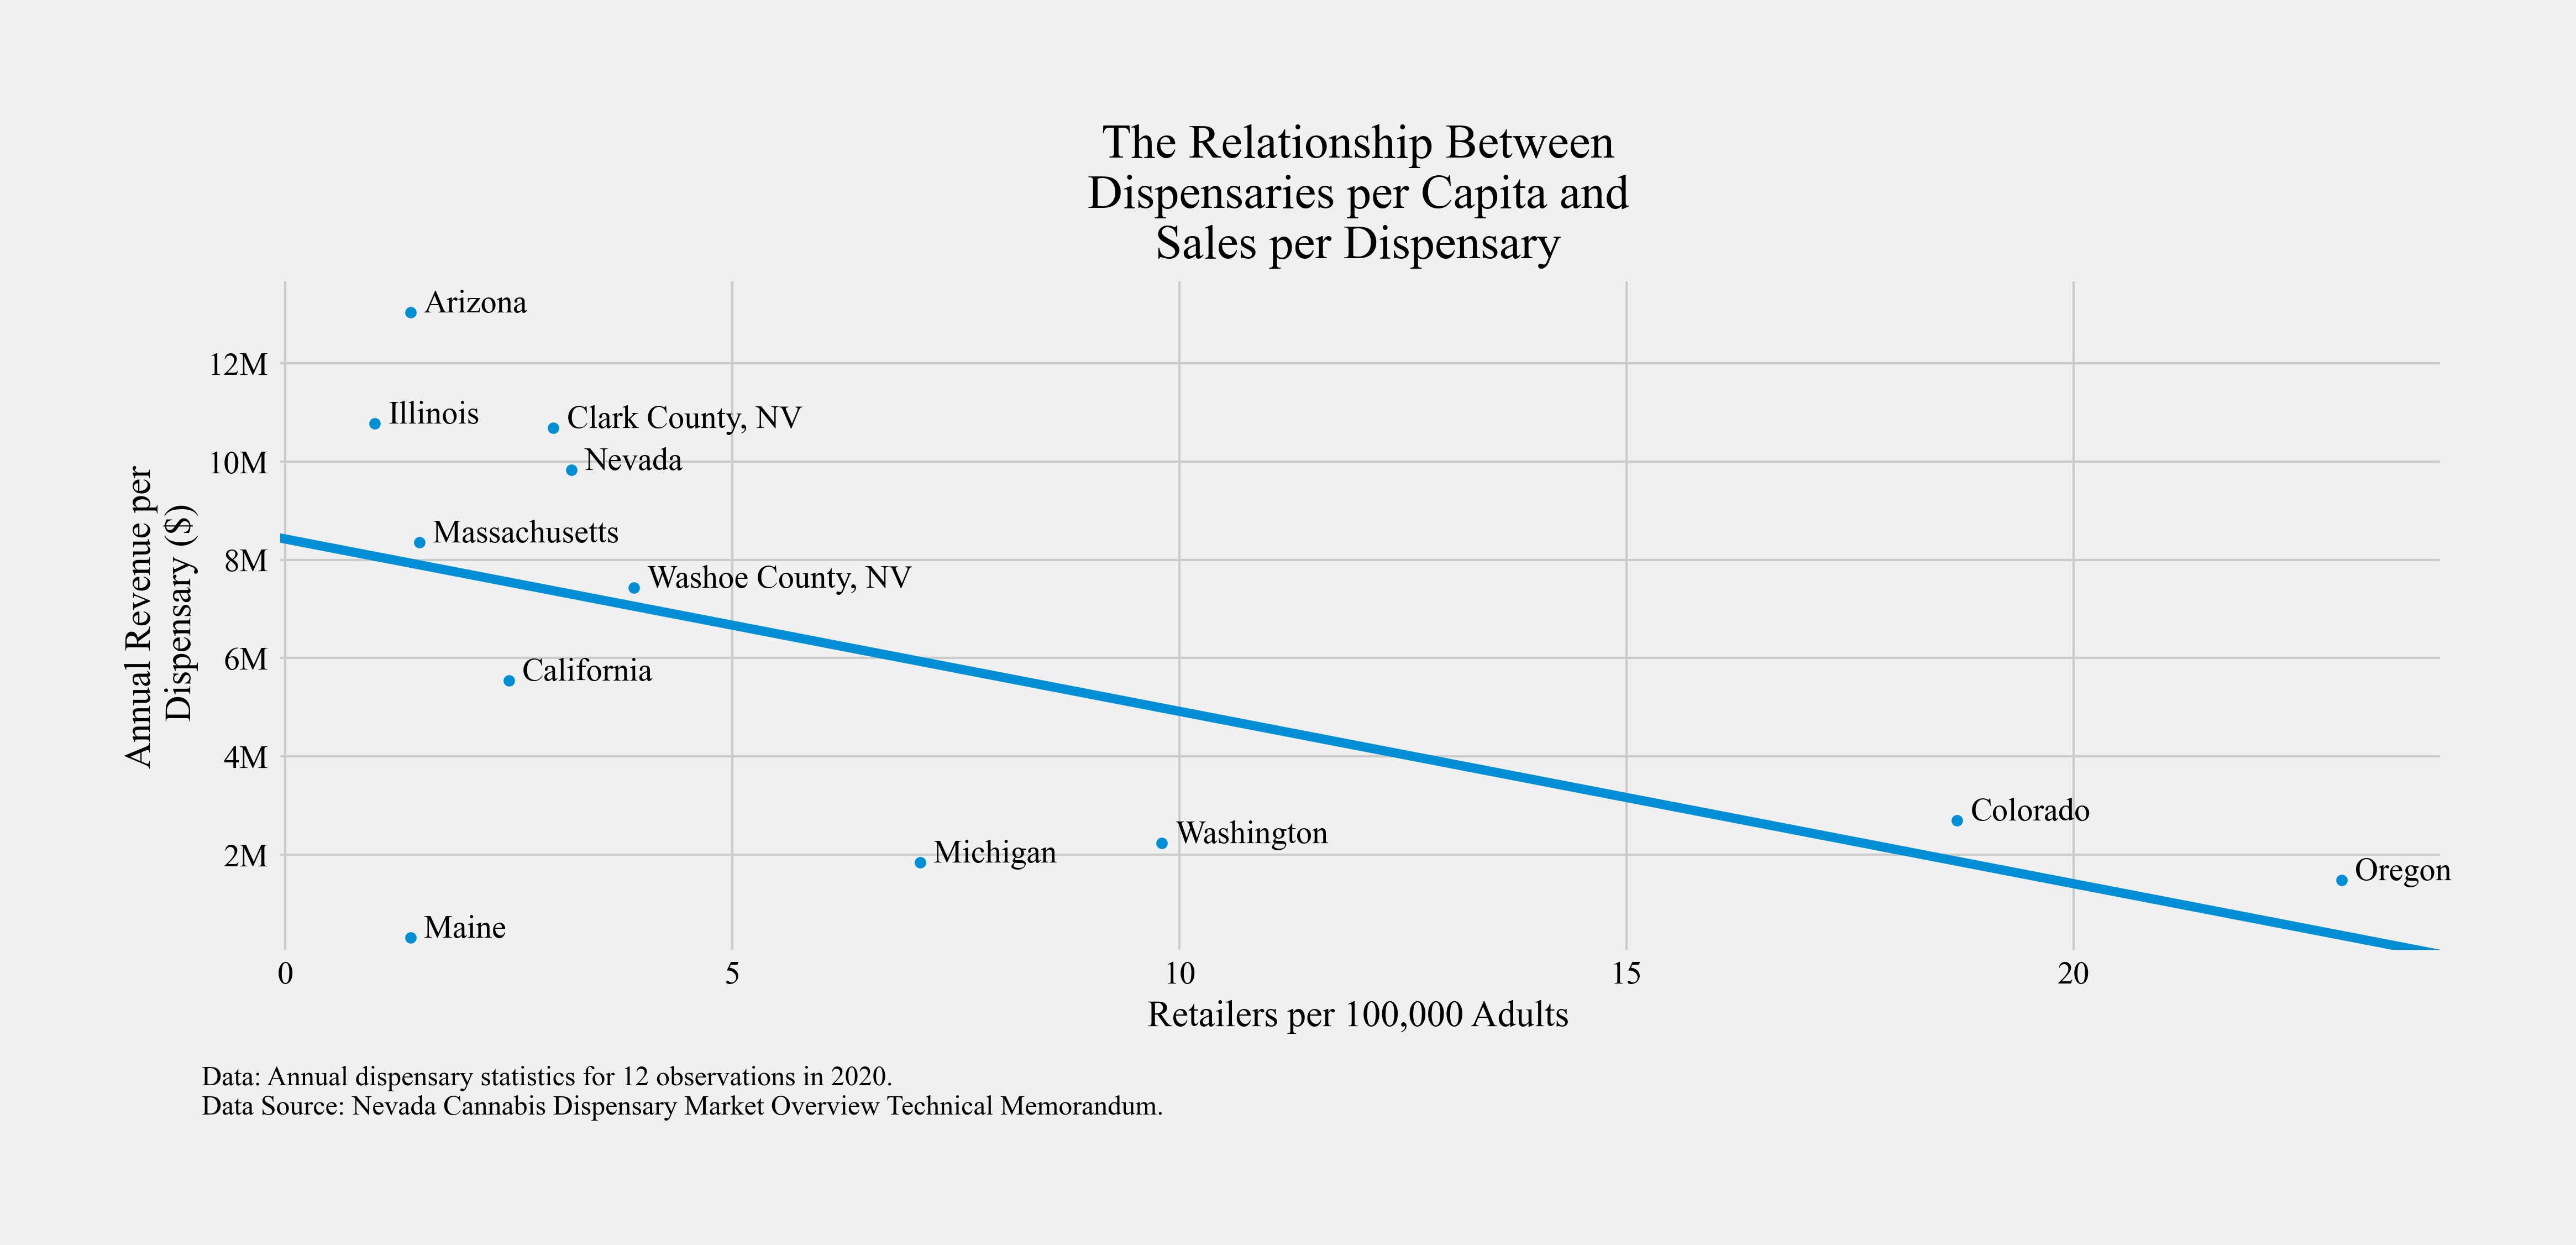
\includegraphics[width=\textwidth]{images/revenue_per_retailer_to_retailers_per_100_000.png}
    \end{subfigure}
    
    \begin{subfigure}[t]{.5\textwidth}
      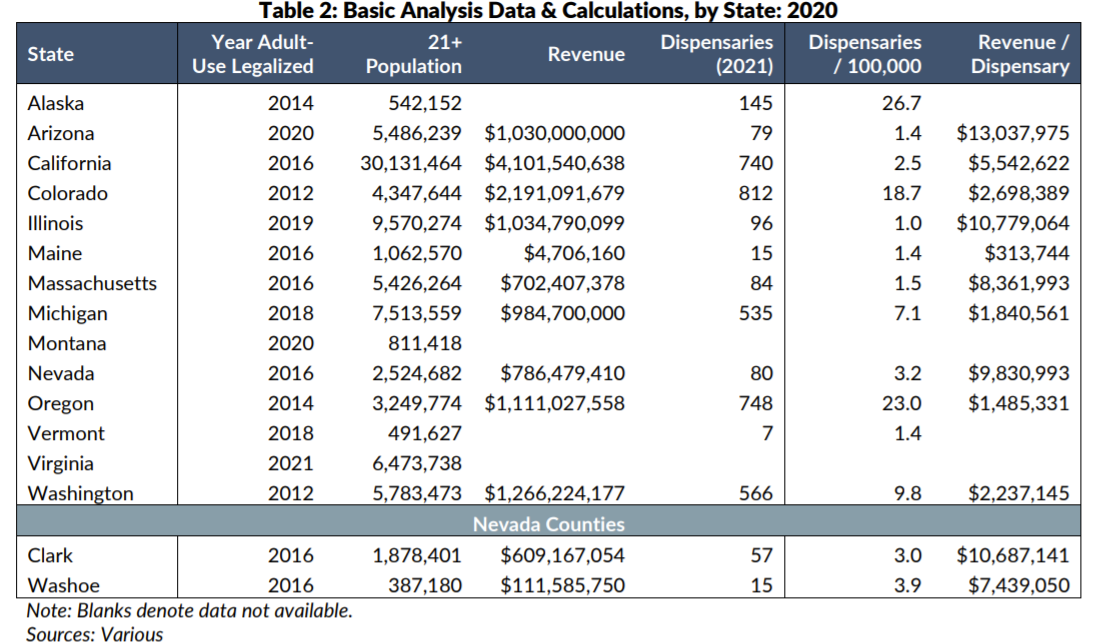
\includegraphics[width=\textwidth]{images/dispensary_statistics.png}
      \caption*{\tiny Source: Nevada Cannabis Dispensary Market Overview Technical Memorandum}
    \end{subfigure}
\end{figure}


\end{frame}
	


%------------------------------------------%
% Research Question
%------------------------------------------%
%\section{Research Question}
%
%\begin{frame}{}
%
%{\large \textbf{Research Question}: What is the relationship between dispensaries per capita and revenue per dispensary?}\vspace{0.5\baselineskip}\\
%
%\begin{figure}
%    \begin{subfigure}[t]{1\textwidth}
%      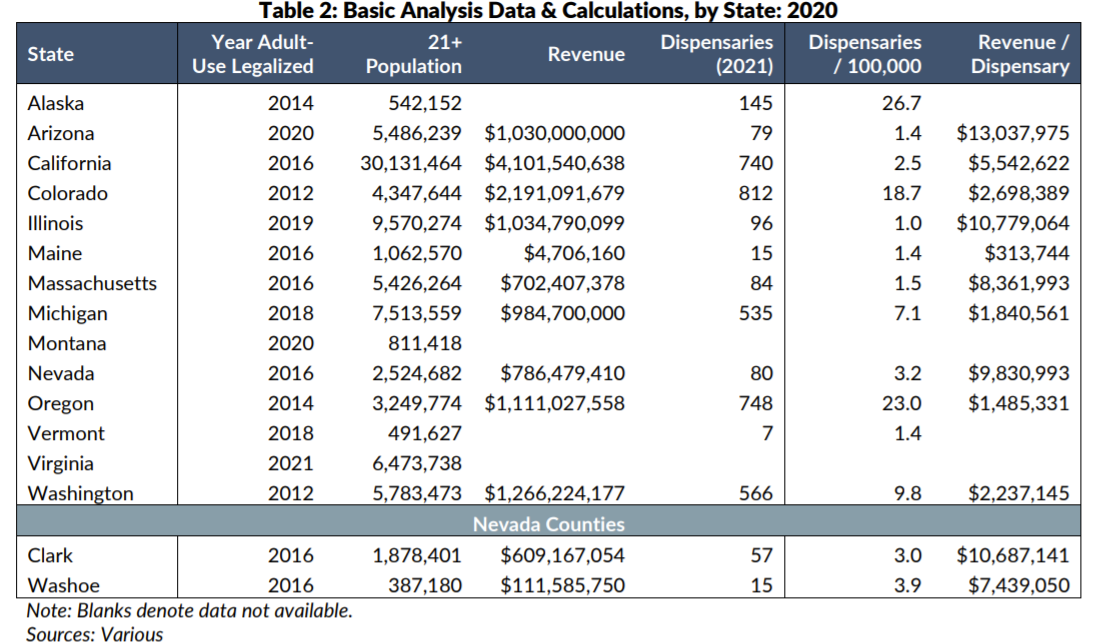
\includegraphics[width=\textwidth]{images/dispensary_statistics.png}
%    \end{subfigure}
%    \caption*{\tiny Source: Nevada Cannabis Dispensary Market Overview Technical Memorandum}
%\end{figure}
%
%\end{frame}

%------------------------------------------%
% Panel Data
%------------------------------------------%


\section{Economic Theory}

% Individuals

\begin{frame}{}

{\large \textbf{How do individuals make decisions at the margin?}}\vspace{0.5\baselineskip}\\

\begin{figure}
    \begin{subfigure}[t]{.4\textwidth}
      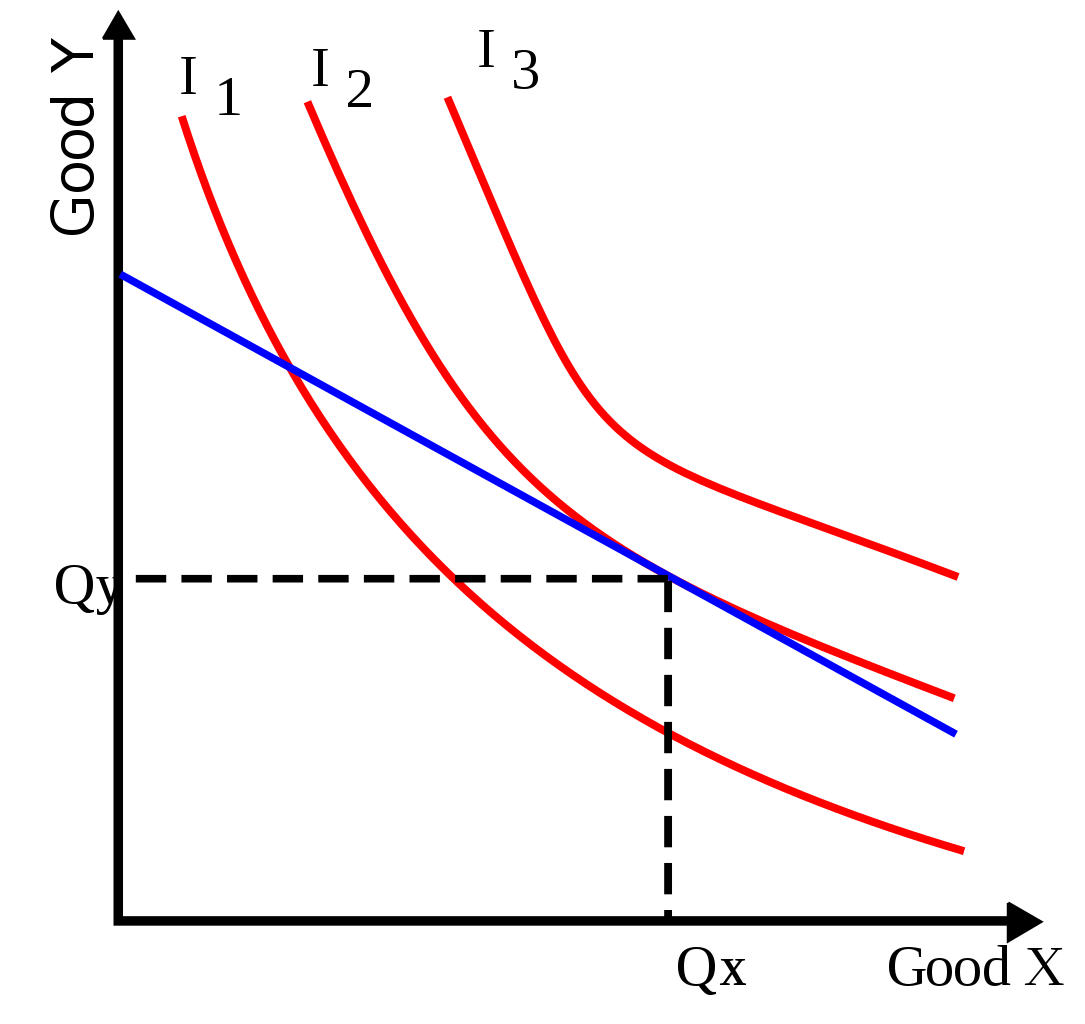
\includegraphics[width=\textwidth]{images/indifference_curves_showing_budget_line.png}
      \caption*{\scriptsize Indifference curves and budget constraints for normal / inferior goods\newline\tiny Source: SilverStar at en.wikipedia}
    \end{subfigure}\hspace{.5in}%
    \begin{subfigure}[t]{.4\textwidth}
      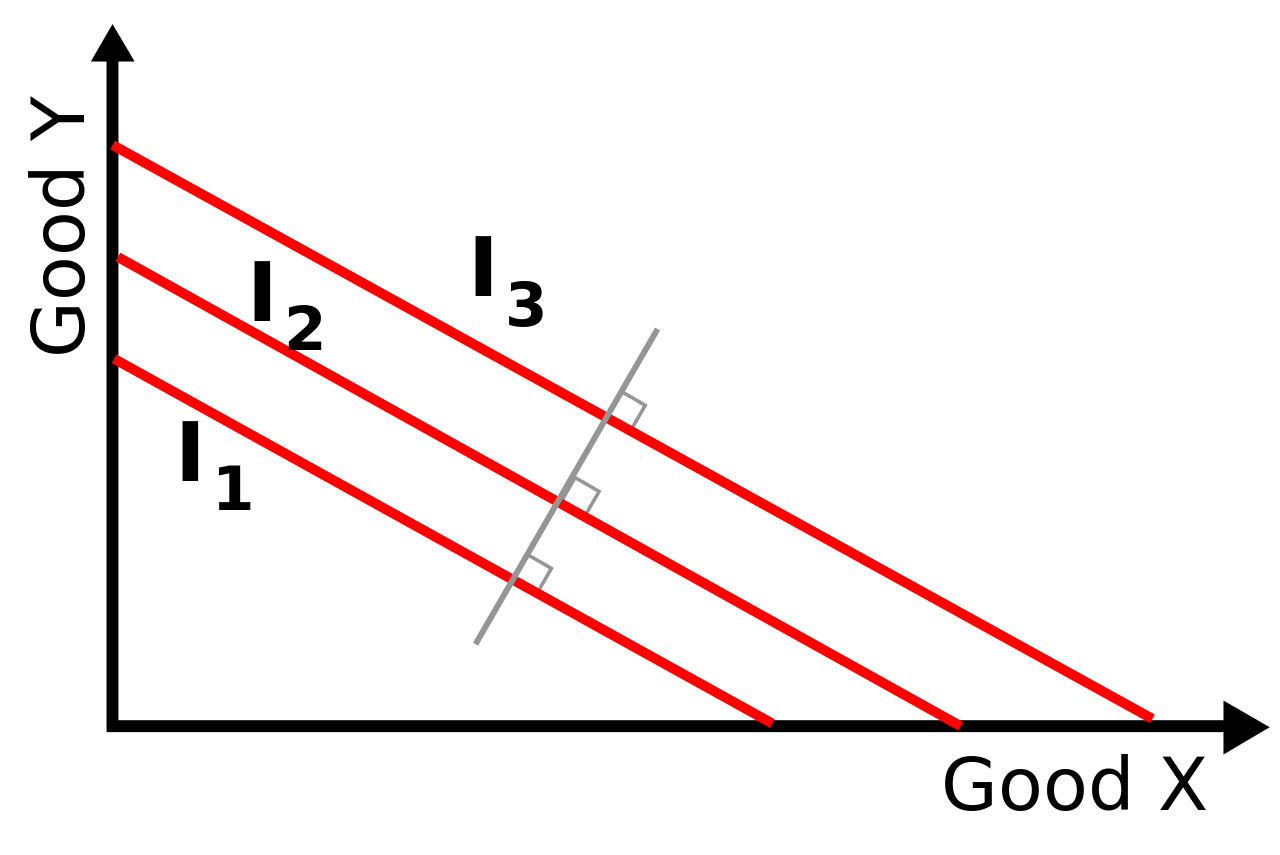
\includegraphics[width=\textwidth]{images/indifference-curves-perfect-substitutes.png}
      \caption*{\scriptsize Indifference ``\textit{curves}'' for perfect substitutes\newline\tiny Source: SilverStar at en.wikipedia}
    \end{subfigure}
    
\end{figure}


\end{frame}

% Competitive Market

\begin{frame}{}

{\large \textbf{What is economic surplus in a competitive market?}}\vspace{0.5\baselineskip}\\

\begin{figure}
    \begin{subfigure}[t]{.4\textwidth}
      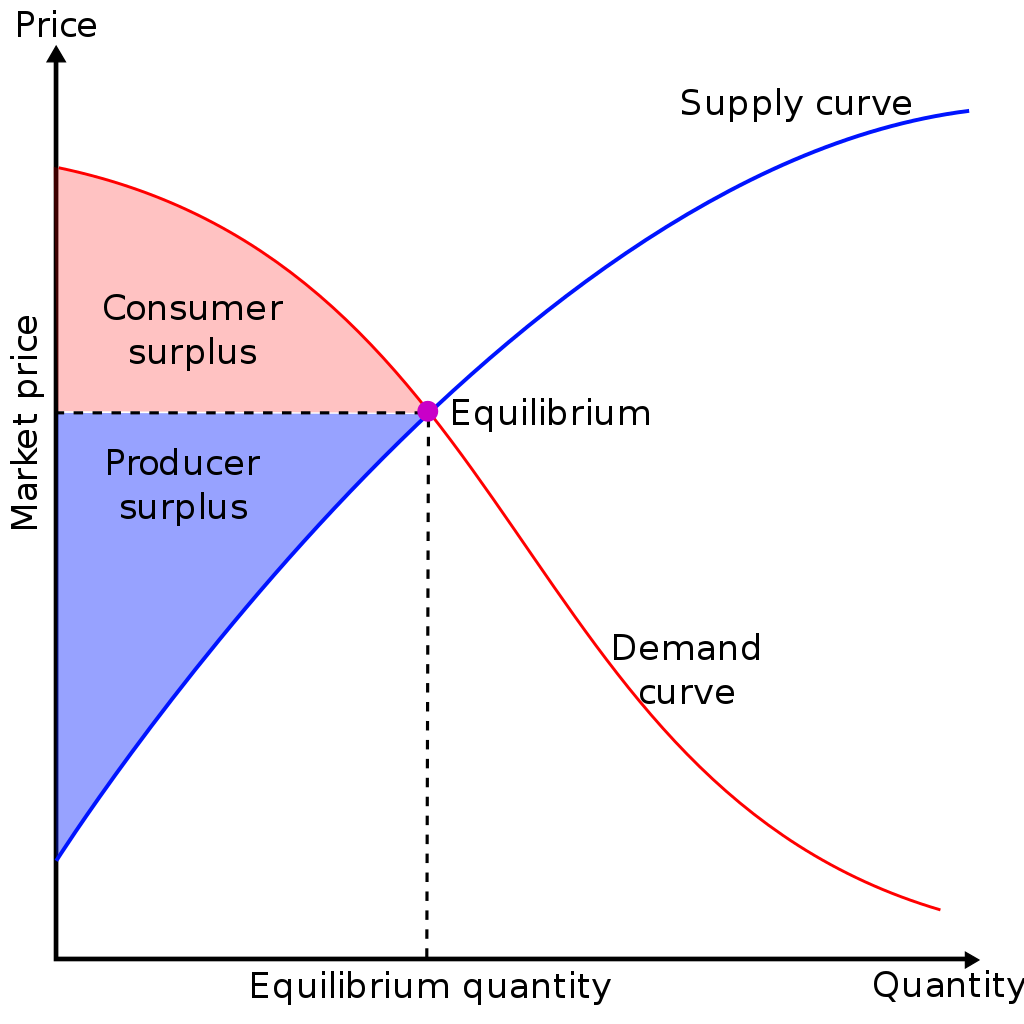
\includegraphics[width=\textwidth]{images/economic-surplus.png}
      \caption*{\scriptsize Economic Surplus in Perfect Competition Equilibrium\tiny \newline Source: SilverStar at en.wikipedia}
    \end{subfigure}\hspace{.5in}
\end{figure}

\vspace{0.5\baselineskip}{\large It depends...!}

\end{frame}

% Tax

\begin{frame}{}

{\large \textbf{Who bears the cost of a tax?}}\vspace{0.5\baselineskip}\\

\begin{figure}
%    \begin{subfigure}[t]{.4\textwidth}
%      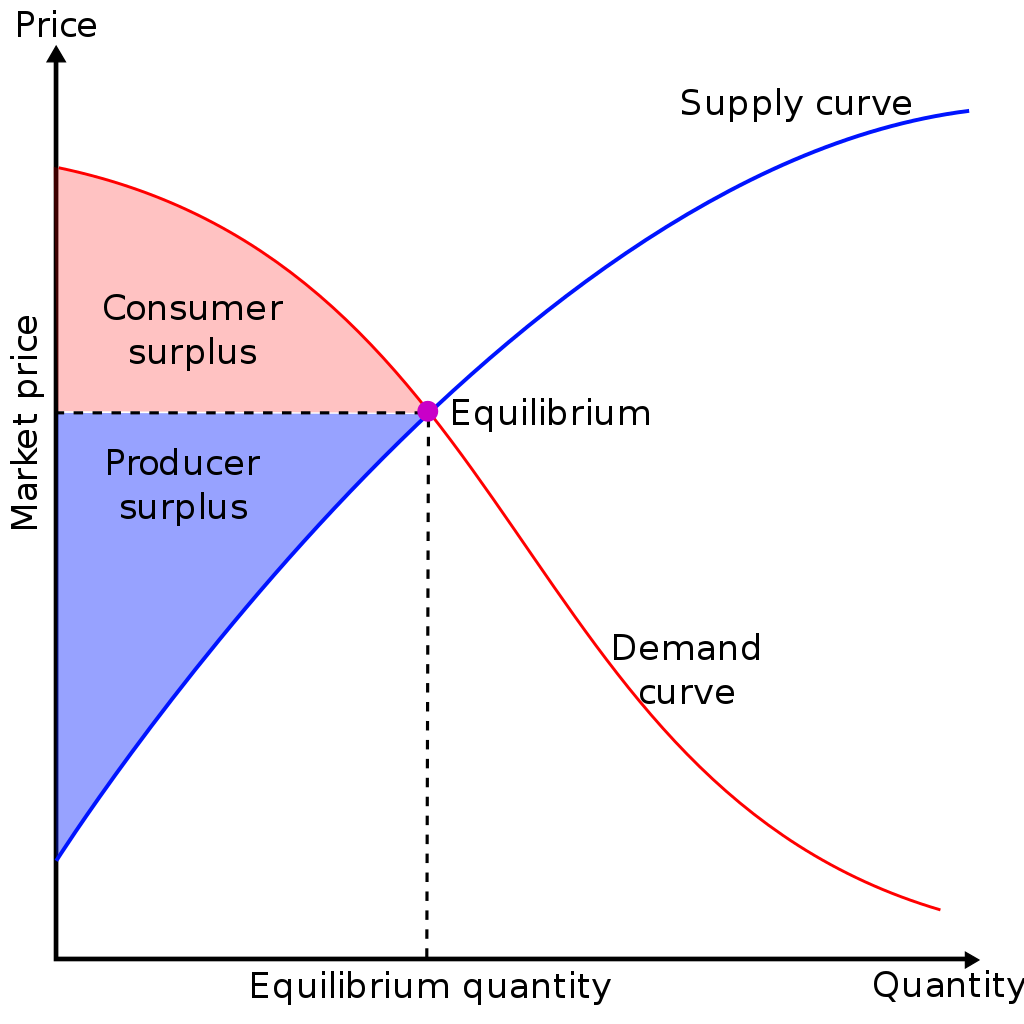
\includegraphics[width=\textwidth]{images/economic-surplus.png}
%      \caption*{\scriptsize Economic Surplus in Perfect Competition Equilibrium\tiny \newline Source: SilverStar at en.wikipedia}
%    \end{subfigure}\hspace{.5in}%
    \begin{subfigure}[t]{.4\textwidth}
      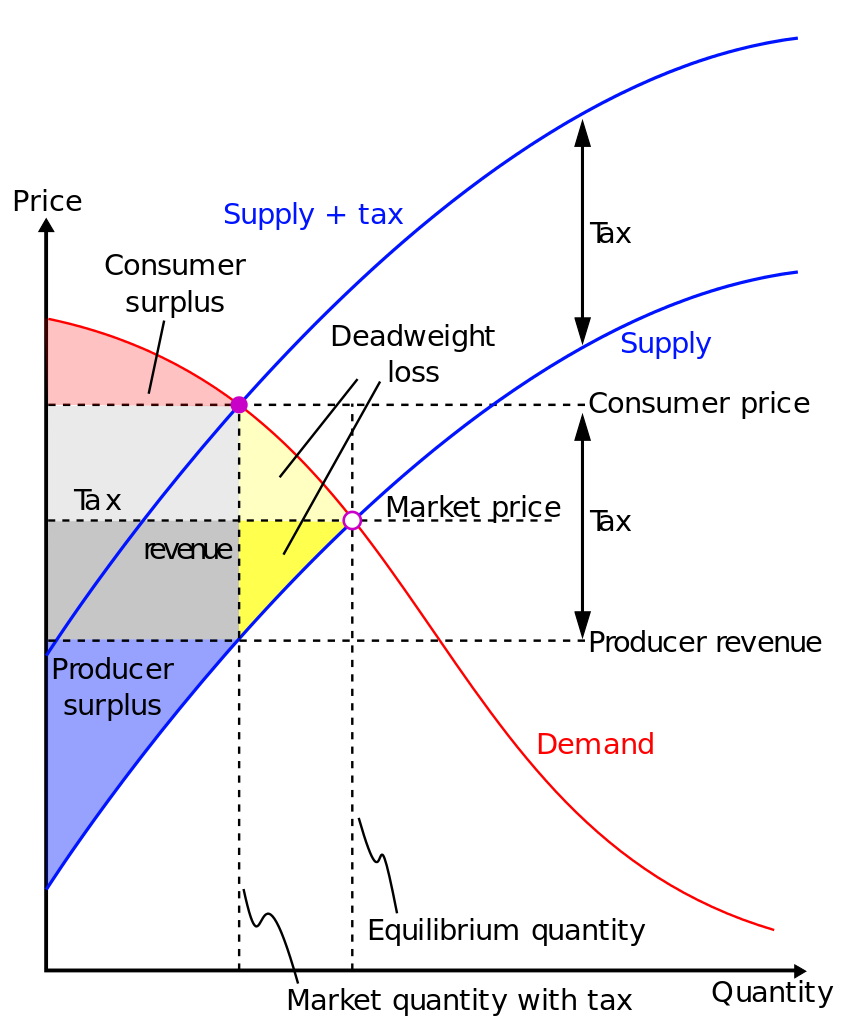
\includegraphics[width=\textwidth]{images/economic-surplus-tax.png}
      \caption*{\scriptsize Effects of a tax on a market\newline\tiny Source: 	SilverStar, Evan Derickson at en.wikipedia}
    \end{subfigure}
    
%\caption*{Effects of a tax on a market\tiny Source: Paul Hield at en.wikipedia}
\end{figure}

\vspace{0.5\baselineskip}{\large It depends...!}


\end{frame}

% Quantity caps.
\begin{frame}{}

{\large \textbf{Who bears the cost of quantity restrictions?}}\vspace{0.5\baselineskip}\\

\begin{figure}
%    \begin{subfigure}[t]{.4\textwidth}
%      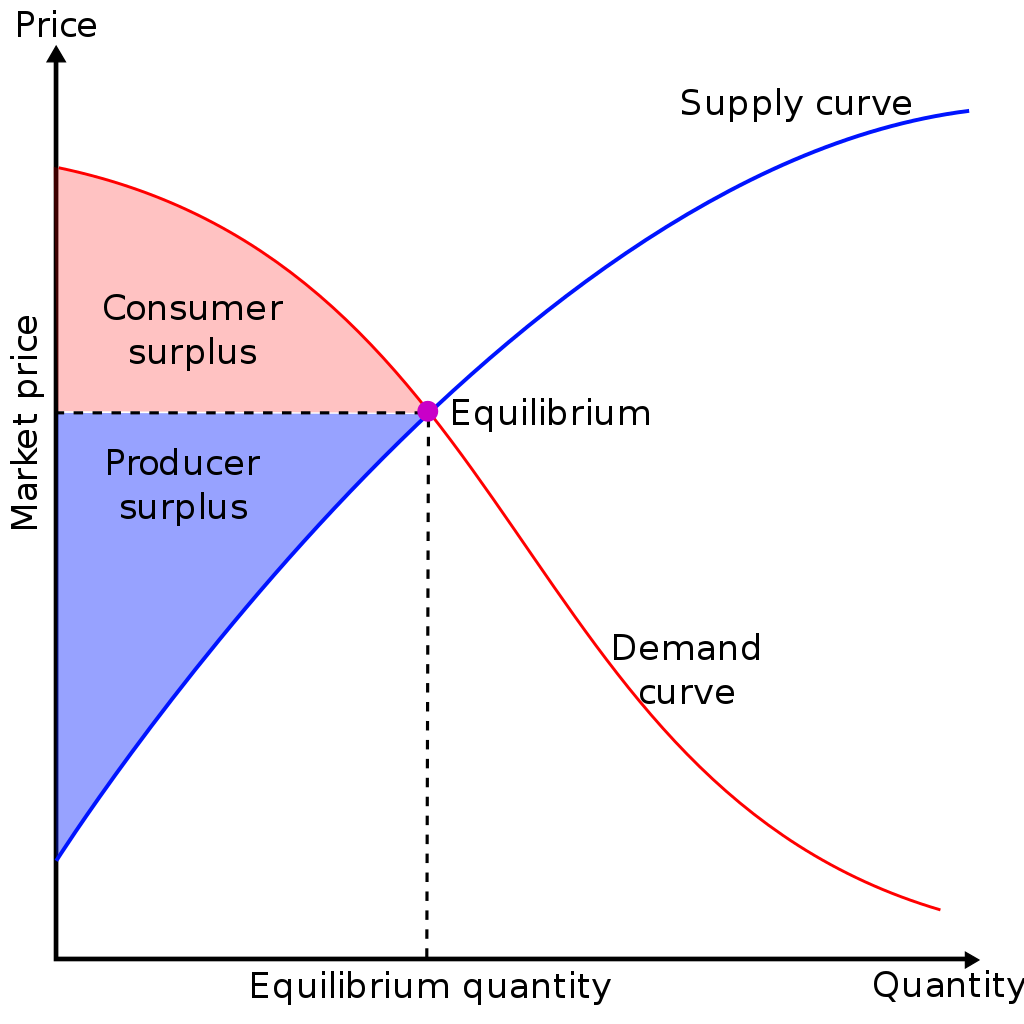
\includegraphics[width=\textwidth]{images/economic-surplus.png}
%      \caption*{\scriptsize Economic Surplus in Perfect Competition Equilibrium\tiny \newline Source: SilverStar at en.wikipedia}
%    \end{subfigure}\hspace{.5in}%
    \begin{subfigure}[t]{.4\textwidth}
      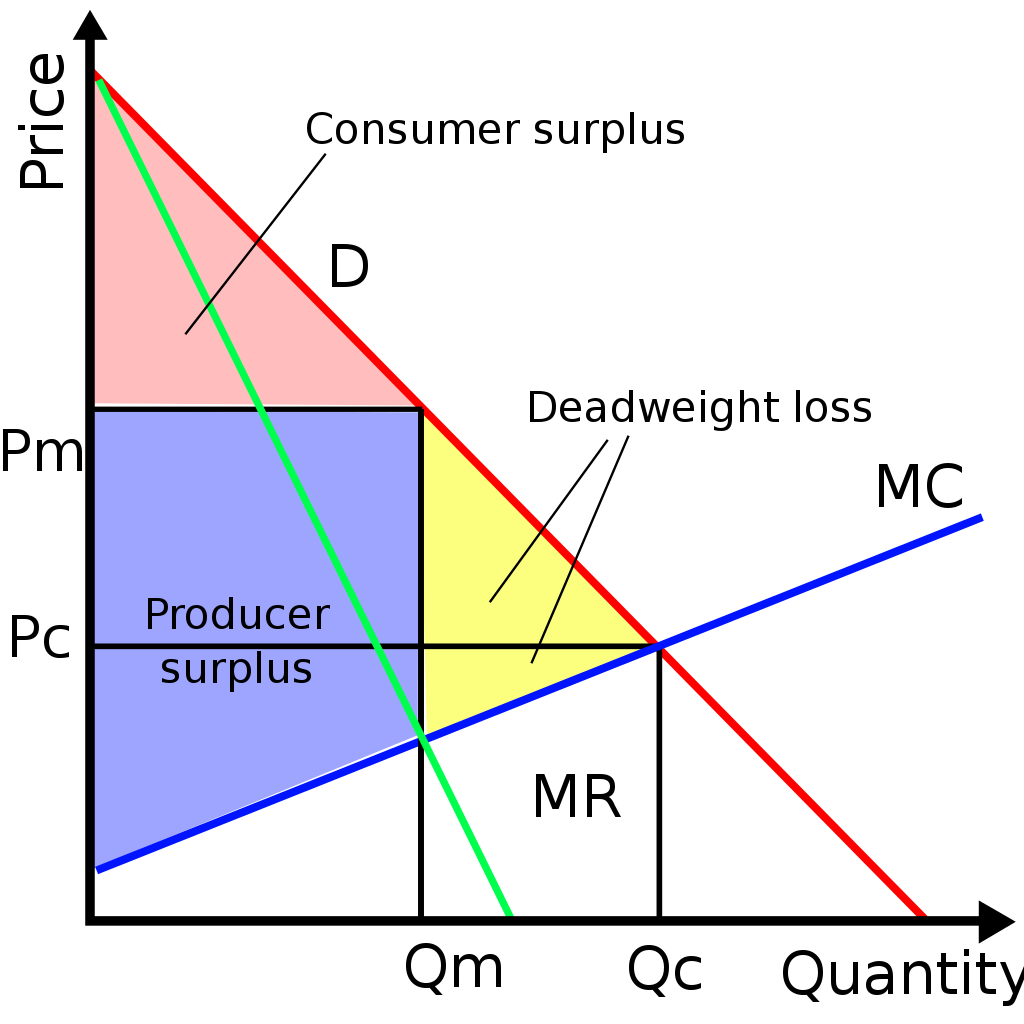
\includegraphics[width=\textwidth]{images/monopoly-surpluses.png}
      \caption*{\scriptsize Effects of a quantity restrictions on a market\newline\tiny Source: 	SilverStar at en.wikipedia}
    \end{subfigure}
\end{figure}

\vspace{0.5\baselineskip}{\large It depends...!}


\end{frame}


%------------------------------------------%
% Panel Data
%------------------------------------------%
\section{Panel Data}

\begin{frame}{}

{\large \textbf{Panel Data}}\vspace{0.5\baselineskip}\\

A panel has the form

\begin{figure}
    \begin{subfigure}[t]{.5\textwidth}
      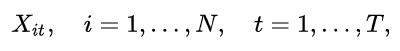
\includegraphics[width=\textwidth]{images/panel.png}
    \end{subfigure}
\end{figure}

where $i$ is the individual dimension and $t$ is the time dimension.\vspace{0.5\baselineskip}\\

A general panel data regression model is written as

\begin{figure}
    \begin{subfigure}[t]{.3\textwidth}
      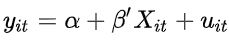
\includegraphics[width=\textwidth]{images/regression.png}
    \end{subfigure}
\end{figure}

where

\begin{figure}
    \begin{subfigure}[t]{.25\textwidth}
      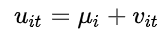
\includegraphics[width=\textwidth]{images/errors.png}
    \end{subfigure}
\end{figure}

Estimation with a \textbf{fixed effects} or \textbf{random effects} model depends on assumptions about $\mu_i$, the individual-specific, time-invariant effects.

\end{frame}


%------------------------------------------%
% Fixed Effects Models
%------------------------------------------%
%\section{Fixed Effects Models}
%
%\begin{frame}{}
%
%{\large \textbf{Fixed Effects Models}}\vspace{0.5\baselineskip}\\
%
%\begin{figure}
%    \begin{subfigure}[t]{1\textwidth}
%      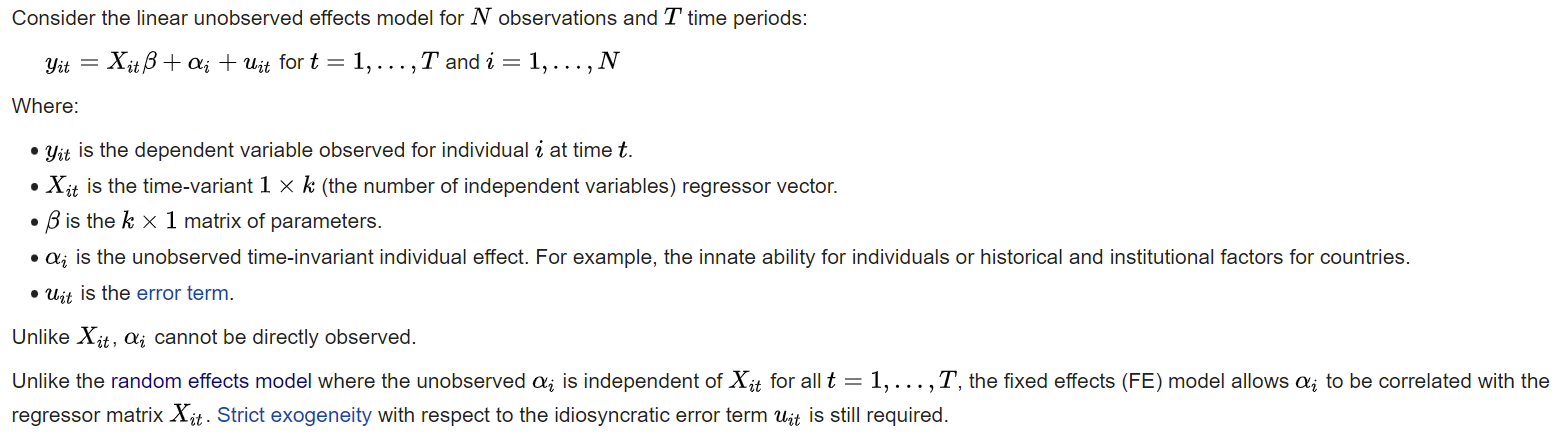
\includegraphics[width=\textwidth]{images/fixed-effects.png}
%    \end{subfigure}
%\end{figure}
%
%\end{frame}


%------------------------------------------%
% Random Effects Models
%------------------------------------------%
%\section{Random Effects Models}
%
%\begin{frame}{}
%
%{\large \textbf{Random Effects Models}}\vspace{0.5\baselineskip}\\
%
%\begin{figure}
%    \begin{subfigure}[t]{1\textwidth}
%      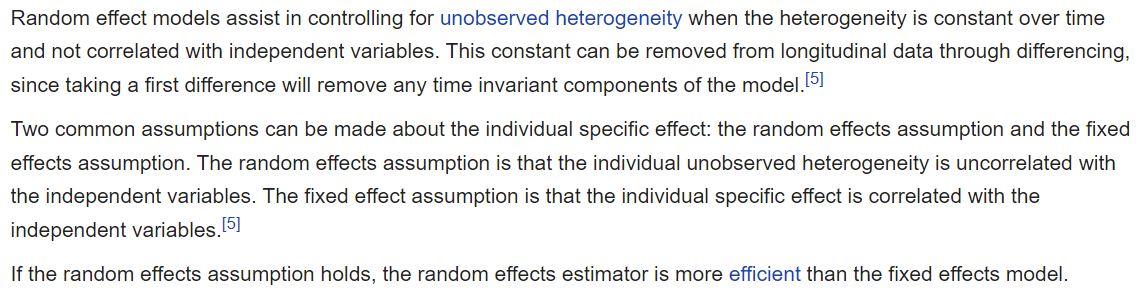
\includegraphics[width=\textwidth]{images/random-effects.png}
%    \end{subfigure}
%\end{figure}
%
%\end{frame}


%------------------------------------------%
% Takeaway
%------------------------------------------%
\section{Conclusion}

\begin{frame}{}

%{\large \textbf{Future work}: Look at geographic distribution of licensees}\vspace{0.5\baselineskip}\\
%
%\begin{figure}
%    \begin{subfigure}[t]{1\textwidth}
%      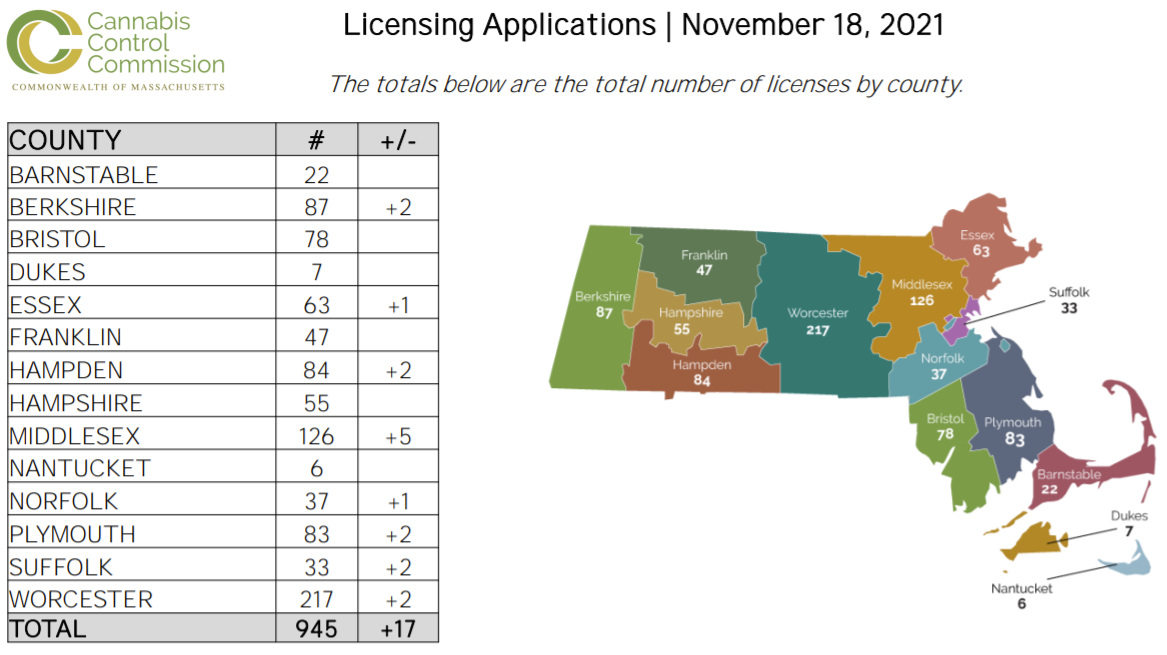
\includegraphics[width=\textwidth]{images/ma_application_map.png}
%    \end{subfigure}
%\end{figure}

\begin{center}
\begin{minipage}{3.85in}

\includegraphics[width=.25in]{images/prayer.png} Thank you for coming.\vspace{0.5\baselineskip}\\


Take some time and discuss any conclusions drawn.
\end{minipage}
\end{center}

\end{frame}

%------------------------------------------%
\end{document}
%------------------------------------------%
